\section{Pi0Reconstruction}

This analyzer is implementing the reconstruction of a $\pi^0$ candidate from two photon candidates
in the Liquid Krypton calorimeter. The eventual reconstructed candidate is then made available to
further analyzer as a \class{KinePart} object. 

The simple algorithm implemented works under strong hypothesis: 
\begin{itemize}
  \item The clusters in LKr are all due to individual photons.
  \item The event contains only a single $\pi^0$ that decayed into two photons, both in the
  acceptance of the LKr.
\end{itemize}
Every cluster is transformed to a photon candidate. The energy being the cluster energy and the
momentum being computed using the reconstructed vertex. Every possible combination of candidate pair
is tried and the pair with the invariant mass closest to $m_{\pi^0}$ is selected to reconstruct the
$\pi^0$. 

\subsection{Pi0Reconstruction implementation}

The first step is to create the skeleton of the new analyzer. This is
automatically done with the framework python script:
\begin{lstlisting}
NA62AnalysisBuilder.py new Pi0Reconstruction
\end{lstlisting}

The source code of the newly created analyzer can be found in
\path{Examples/include/Pi0Reconstruction.hh} and \path{Examples/src/Pi0Reconstruction.cc}.
Every standard method of the analyzer and each section of code will be described thereafter.

\subsubsection{Constructor}
As this analyzer only needs information from the LKr, this is the only requested TTree. The
analyzer will run some acceptance checks as well and need access to the global instance of the
\class{DetectorAcceptance} object:

\begin{lstlisting}
RequestTree("LKr", new TRecoLKrEvent);
fDetectorAcceptanceInstance = GetDetectorAcceptanceInstance();
\end{lstlisting}

Without forgetting to include the header for the LKr reconstructed events

\begin{lstlisting}
#include "TRecoLKrEvent.hh"
\end{lstlisting}


\subsubsection{InitHist}
In this method all the histograms that will be needed during the processing are created and
registered to the framework:

\begin{itemize}
  \item Histograms for the photon candidates reconstructed energy 
\begin{lstlisting}
BookHisto("g1Energy", 
		new TH1I("G1Energy", "Energy of g1", 100, 0, 75000));
BookHisto("g2Energy", 
		new TH1I("G2Energy", "Energy of g2", 100, 0, 75000));
\end{lstlisting}
	\item 2D histograms to compare reconstructed photon candidates energy with the true Monte Carlo
	energy
\begin{lstlisting}
BookHisto("g1Reco", 
		new TH2I("g1Reco", "g1 Reco vs. Real", 100, 0, 75000, 100, 0, 75000));
BookHisto("g2Reco", 
		new TH2I("g2Reco", "g2 Reco vs. Real", 100, 0, 75000, 100, 0, 75000));
\end{lstlisting}
	\item 2D histograms to compare the reconstructed photon candidates positions on LKr with the
	extrapolated position of the true MC photons
\begin{lstlisting}
BookHisto("g1px", 
		new TH2I("g1px", "g1 px Reco vs. Real", 200, 0, 2000, 200, 0, 2000));
BookHisto("g2px", 
		new TH2I("g2px", "g2 px Reco vs. Real", 200, 0, 2000, 200, 0, 2000));
BookHisto("g1py", 
		new TH2I("g1py", "g1 py Reco vs. Real", 200, 0, 2000, 200, 0, 2000));
BookHisto("g2py", 
		new TH2I("g2py", "g2 py Reco vs. Real", 200, 0, 2000, 200, 0, 2000));
BookHisto("g1pz", 
		new TH2I("g1pz", "g1 pz Reco vs. Real", 10, 240000, 250000, 10, 240000, 250000));
BookHisto("g2pz", 
		new TH2I("g2pz", "g2 pz Reco vs. Real", 10, 240000, 250000, 10, 240000, 250000));
\end{lstlisting}
	\item Histograms for the reconstructed $\pi^0$ candidate properties
\begin{lstlisting}
BookHisto("pi0Energy", 
		new TH1I("pi0Energy", "Energy of pi0", 100, 0, 75000));
BookHisto("pi0Mass", 
		new TH1I("pi0Mass", "Reconstructed mass of pi0", 200, 0, 200));
\end{lstlisting}
	\item Histograms for LKr Monitoring
\begin{lstlisting}
BookHisto("clusterPosition", 
		new TH2I("clusterPosition", 
				"Cluster position on LKr", 500, -2000, 2000, 500, -2000, 2000));
BookHisto("photonsNbr", 
		new TH1I("photonsNbr", "Photons number/event", 10, 0, 10));
BookHisto("energyCalib", 
		new TGraph());
BookHisto("g1EnergyFraction", 
		new TH1I("g1EnergyFraction", 
				"Fraction between real energy and reco energy",	1000, 0, 100));
BookHisto("g2EnergyFraction", 
		new TH1I("g2EnergyFraction", 
				"Fraction between real energy and reco energy",	1000, 0, 100));
\end{lstlisting}
	\item Histograms for the pair selection algorithm
\begin{lstlisting}
BookHisto("gPairSelected", 
		new TH1I("gPairSelected", "Pair of gamma selected for Pi0", 10, 0, 10));
\end{lstlisting}
	\item Histograms specific to Monte Carlo events
\begin{lstlisting}
BookHisto("g1FirstVol", 
		new TH1I("g1FirstVol", "First touched volume for g1", 15, 0, 15));
BookHisto("g2FirstVol", 
		new TH1I("g2FirstVol", "First touched volume for g2", 15, 0, 15));
BookHisto("pdgID", 
		new TH1I("pdgID", "Non complete events : pdgID", 0, 0, 0));
\end{lstlisting}
\end{itemize}

\subsubsection{InitOutput}
This analyzer should provide further analyzers with a $\pi^0$ candidate if any is found. The output
object is first declared in the header:

\begin{lstlisting}
KinePart pi0;
\end{lstlisting}

And then registered in the framework under the name \refcode{pi0} in the \method{InitOutput}
method. It should be noted that to avoid collisions between independent analyzers, this name is
automatically prepended with the name of the analyzer and a dot. In this case, to access this
object from another analyzer, one will have to request \refcode{Pi0Reconstruction.pi0}
\begin{lstlisting}
RegisterOutput("pi0", &pi0);
\end{lstlisting}

\subsubsection{DefineMCSimple}
In this method, the specific event signature $K^+\to\pi^+X\pi^0\to\gamma\gamma X$ is defined where
$X$ can be any kind and any number (including 0) of additional particle. This will allow to do
extra-processing to assess the performances of the analyzer when running on this kind of
simulated events.
\begin{lstlisting}
int kID = fMCSimple->AddParticle(0, 321); //ask for beam Kaon
fMCSimple->AddParticle(kID, 211); //ask for positive pion from initial kaon decay
int pi0ID = fMCSimple->AddParticle(kID, 111); //ask for positive pion from initial kaon decay
fMCSimple->AddParticle(pi0ID, 22); //ask for positive pion from initial kaon decay
fMCSimple->AddParticle(pi0ID, 22); //ask for positive pion from initial kaon decay
\end{lstlisting}


\subsubsection{Process}
All the necessary variables are first declared
\begin{lstlisting}
//Temporary variables
vector<KinePart*> photons;
KinePart *part;
TRecoLKrCandidate *lkrCand;
vector<pair<KinePart*, KinePart*> > candidates;
int i;

//Maps
map<double, int> photonOrder;
map<double, int>::reverse_iterator photonIt, photonIt2;
multimap<double, int> cID;
multimap<double, int>::iterator cIDIterator;

//For input from VertexCDA
TVector3 vertex, direction;
OutputState state;


//Variables for reconstruction
int LKrStartPos = 240413;
KinePart *g1,*g2;
double pi0Mass;
int iLead=-1;
int iTrail=-1;

//Variables for MC checks
double g1EnergyFrac = 0;
double g2EnergyFrac=0;
DetectorAcceptance::volume g1Vol, g2Vol;
bool g1LKr, g2LKr;
TVector3 g1reco, g2reco, g1real, g2real;
\end{lstlisting}

The event is retrieved from the LKr TTree and two calibration constants are declared for the LKr
cluster energy correction:
\begin{lstlisting}
//Get LKr event from TTree
TRecoLKrEvent *LKrEvent = (TRecoLKrEvent*)GetEvent("LKr");
//Calibration constants
double calibMult = 0.9744;
double calibConst = -366.5;
\end{lstlisting}

As stated previously some supplementary work can be done if running on specific Monte Carlo events.
The use of simulated events is not enforced but the \var{withMC} flag is set accordingly:
\begin{lstlisting}
bool withMC = true;
if(fMCSimple.fStatus == MCSimple::kMissing){
	for(int i=0; i<MCTruthEvent->GetNKineParts(); i++){
		FillHisto("pdgID", 
				((KinePart*)MCTruthEvent->GetKineParts()->At(i))->GetParticleName(), 1);
	}
	return;
}
if(fMCSimple.fStatus == MCSimple::kEmpty) withMC = false;
\end{lstlisting}

The vertex is required to reconstruct the photons momenta and is retrieved from the
\class{VertexCDA} analyzer and its validity if verified.
\begin{lstlisting}
//Get vertex from VertexCDA analyzer
vertex = *(TVector3*)GetOutput("VertexCDA.Vertex", state);
//Check we got the vertex. We cannot work without the vertex
if(state!=kOValid) return;
\end{lstlisting}

Then all the LKr clusters are transformed into photon candidates. The hypothesis is made that all
clusters are due to a photon and that they all originate from the vertex. In which case the
particle momenta is 
$\vec{p}=E_{cl}*\frac{(\vec{x}_{cl}-\vec{V})}{\left|\vec{x}_{cl}-\vec{V}\right|}$ where $E_{cl}$ is
the corrected cluster energy, $\vec{x}_{cl}$ is the position of the cluster on the LKr surface and
$\vec{V}$ is the vertex. The processing can only continue if at least two photons candidates are
found.
\begin{lstlisting}
//Loop over the LKr clusters and create a KinePart photon candidate
for(int i=0; i<LKrEvent->GetNCandidates(); i++){
	lkrCand = (TRecoLKrCandidate*)LKrEvent->GetCandidate(i);
	part = new KinePart();
	//Fill the cluster position histogram
	FillHisto("clusterPosition", 
			lkrCand->GetClusterX()*10, lkrCand->GetClusterY()*10);
	//Set the LKr position (*10 to go from cm to mm)
	direction.SetXYZ(lkrCand->GetClusterX()*10, 
					lkrCand->GetClusterY()*10, LKrStartPos);
	//Set the direction
	direction = direction - vertex;
	//Set the magnitude of the direction to the corrected cluster energy to form the momentum (photon hypothesis)
	direction.SetMag(lkrCand->GetClusterEnergy()*1000*calibMult + calibConst);
	//Assign the properties to the KinePart
	part->SetProdPos(TLorentzVector(vertex, 0));
	part->SetInitialMomentum(direction);
	part->SetInitialEnergy(lkrCand->GetClusterEnergy()*1000*calibMult + calibConst);
	//Push the candidate in the list
	photonOrder.insert(pair<double, int>(
		lkrCand->GetClusterEnergy()*1000*calibMult + calibConst, photons.size()));
	photons.push_back(part);
}
//Fill the photon multiplicity histogram
FillHisto("photonsNbr", photonOrder.size());

i=0;
//We need at leat 2 photons to reconstruct the pi0
if(photonOrder.size()>=2){
\end{lstlisting}

In most of the case more than two photon candidates are found. This is mainly due to the
contribution of the charged pion creating a cluster and the photons sometimes creating more than one
cluster. The ratio between the invariant mass of every possible photon candidate pair and the
$\pi^0$ mass is computed. The invariant mass is computed as $M = \sqrt{p_{g_1}^2 + p_{g_2}^2}$ where
$p_{g_{1,2}}$ are the quadri-momenta of the photon candidates. The pair whose ratio is closest to 1
(the pair with the invariant mass closest to the $\pi^0$ mass) is chosen.
\begin{lstlisting}
//Looping over possible photon pairs and computing invariant mass for each
photonIt2 = photonOrder.rbegin();
for(photonIt = photonOrder.rbegin(); photonIt != photonOrder.rend(); photonIt++){
	g1 = photons[photonIt->second];
	photonIt2 = photonIt;
	for(photonIt2++; photonIt2 != photonOrder.rend(); photonIt2++){
		g2 = photons[photonIt2->second];

		candidates.push_back(pair<KinePart*, KinePart*>(g1, g2));
		pi0Mass = sqrt(pow(g1->GetInitialEnergy() + g2->GetInitialEnergy(),2)
					 - (g1->GetInitialMomentum() + g2->GetInitialMomentum()).Mag2());
		//insert the invariant mass divided by the pi0 mass in the map
		cID.insert(pair<double, int>(fabs((pi0Mass/134.9766)-1), i));
		i++;
	}
}
//Select the photon pair closest to the pi0 mass
FillHisto("gPairSelected", cID.begin()->second);
g1 = candidates[cID.begin()->second].first;
g2 = candidates[cID.begin()->second].second;
\end{lstlisting}

If Monte Carlo data is available the energy of the selected photon candidates are compared with the
simulated photons coming from the $\pi^0$ decay. Tests are also done to see whether they are in the
acceptance of the LKr or not. 
\begin{lstlisting}
//Are we working with MC?
if(withMC){

	//Select the most energetic photons coming from the pi0 decay
	if(fMCSimple["gamma"][0]->GetInitialEnergy() >= fMCSimple["gamma"][1]->GetInitialEnergy()) iLead = 0;
	else iLead = 1;
	iTrail = !iLead;

	//Compare the energy with the selected pair
	g1EnergyFrac = g1->GetInitialEnergy()/fMCSimple["gamma"][iLead]->GetInitialEnergy();
	g2EnergyFrac = g2->GetInitialEnergy()/fMCSimple["gamma"][iTrail]->GetInitialEnergy();

	//Are the 2 real photons in the LKr acceptance?
	fDetectorAcceptanceInstance->FillPath(fMCSimple["gamma"][iLead]->GetProdPos().Vect(), fMCSimple["gamma"][iLead]->GetInitialMomentum());
	g1Vol = fDetectorAcceptanceInstance->FirstTouchedDetector();
	g1LKr = fDetectorAcceptanceInstance->GetDetAcceptance(DetectorAcceptance::kLKr);
	fDetectorAcceptanceInstance->CleanDetPath();
	fDetectorAcceptanceInstance->FillPath(fMCSimple["gamma"][iTrail]->GetProdPos().Vect(), fMCSimple["gamma"][iTrail]->GetInitialMomentum());
	g2Vol = fDetectorAcceptanceInstance->FirstTouchedDetector();
	g2LKr = fDetectorAcceptanceInstance->GetDetAcceptance(DetectorAcceptance::kLKr);

	FillHisto("g1FirstVol", g1Vol);
	FillHisto("g2FirstVol", g2Vol);
}
\end{lstlisting}

If no Monte Carlo are available the photons are simply assumed to be in the LKr acceptance and the
rest of the processing is only done if the photons are inside LKr.
\begin{lstlisting}
else{
	g1Vol = DetectorAcceptance::kLKr;
	g2Vol = DetectorAcceptance::kLKr;
	g1LKr = true;
	g2LKr = true;
}

if( (g1Vol != DetectorAcceptance::kLAV && g1LKr == true)
	&& (g2Vol != DetectorAcceptance::kLAV && g2LKr == true)){
\end{lstlisting}

Again if simulated data are available, the positions of the simulated photons are extrapolated at
the LKr surface and compared with the selected candidates and the comparison histograms are filled.
\begin{lstlisting}
//Expected position on LKr
g1reco = propagate(g1->GetProdPos().Vect(), g1->GetInitialMomentum(), LKrStartPos);
g2reco = propagate(g2->GetProdPos().Vect(), g2->GetInitialMomentum(), LKrStartPos);

if(withMC){
	//Comparison reconstructed momenta and energies between reconstructed and real
	g1real = propagate(fMCSimple["gamma"][iLead]->GetProdPos().Vect(), fMCSimple["gamma"][iLead]->GetInitialMomentum(), LKrStartPos);
	g2real = propagate(fMCSimple["gamma"][iTrail]->GetProdPos().Vect(), fMCSimple["gamma"][iTrail]->GetInitialMomentum(), LKrStartPos);

	FillHisto("g1px", g1reco.X(), g1real.X());
	FillHisto("g2px", g2reco.X(), g2real.X());
	FillHisto("g1py", g1reco.Y(), g1real.Y());
	FillHisto("g2py", g2reco.Y(), g2real.Y());
	FillHisto("g1pz", g1reco.Z(), g1real.Z());
	FillHisto("g2pz", g2reco.Z(), g2real.Z());
	FillHisto("g1Reco", g1->GetInitialEnergy(), fMCSimple["gamma"][iLead]->GetInitialEnergy());
	FillHisto("g2Reco", g2->GetInitialEnergy(), fMCSimple["gamma"][iTrail]->GetInitialEnergy());
	//Dont do it if we are likely to have selected the wrong photon
	if(g1EnergyFrac>0.95) FillHisto("energyCalib", g1->GetInitialEnergy(), fMCSimple["gamma"][iLead]->GetInitialEnergy());
	if(g2EnergyFrac>0.95) FillHisto("energyCalib", g2->GetInitialEnergy(), fMCSimple["gamma"][iTrail]->GetInitialEnergy());
	FillHisto("g1EnergyFraction", g1EnergyFrac);
	FillHisto("g2EnergyFraction", g2EnergyFrac);
}

FillHisto("g1Energy", g1->GetInitialEnergy());
FillHisto("g2Energy", g2->GetInitialEnergy());
\end{lstlisting}

Finally the $\pi^0$ candidate is reconstructed. Its energy is the sum of the photons energies and
its momentum  is the sum of the photon momenta. The state of the output is set as \refcode{kOValid}
to signal further analyzer that the output can be used. The histograms corresponding to the $\pi^0$
candidate values are filled.
\begin{lstlisting}
//Reconstruct the pi0 candidate and create the KinePart
pi0.SetInitialEnergy(g1->GetInitialEnergy() + g2->GetInitialEnergy());
direction = g1->GetInitialMomentum();
direction.SetMag(g1->GetInitialEnergy());
g1->SetInitialMomentum(direction);
direction = g2->GetInitialMomentum();
direction.SetMag(g2->GetInitialEnergy());
g2->SetInitialMomentum(direction);
pi0.SetInitialMomentum(g1->GetInitialMomentum() + g2->GetInitialMomentum());

//Set the output state as valid (we have a candidate)
SetOutputState("pi0", kOValid);

//Fill the pi0 histograms
FillHisto("pi0Energy", pi0.GetInitialEnergy());
FillHisto("pi0Mass", sqrt(pow(pi0.GetInitialEnergy(),2) - pi0.GetInitialMomentum().Mag2()));
\end{lstlisting}


The last step is to release all the memory that has been allocated during the processing. This can
safely be done here as this memory is not part of the output. If memory had been allocated for the
output, the release would have been done in the \method{PostProcess} method.
\begin{lstlisting}
//Delete all the created KinePart
while(photons.size()>0){
	delete photons.back();
	photons.pop_back();
}
\end{lstlisting}

\subsubsection{PostProcess}
This method is meant to destroy temporary objects that have been allocated during \method{Process}
and that shall be destroyed only after all the analyzers finished processing the event. This is
typically the case for memory allocated for the output of the analyzer. In the specific case of this
analyzer, no such memory has been allocated and this method will stay empty.

\subsubsection{ExportPlot}
All the histograms previously booked with \method{BookHisto} are saved in the output ROOT file with

\begin{lstlisting}
SaveAllPlots();
\end{lstlisting} 

\subsubsection{DrawPlot}
Similarly if the analysis is running in graphical mode, all the histograms previously booked with
\method{BookHisto} should be displayed on screen:

\begin{lstlisting}
DrawAllPlots();
\end{lstlisting} 

\subsection{Results}
The figure \ref{pi0validation} shows some results of this analyzer run on simulated
$K^+\to\pi^+\pi^0\to\gamma\gamma$ events. The top plots shows the reconstructed energy of the
$\pi^0$ candidate when found and the invariant mass of the photon pair being selected as decay
product of the $pi^0$. The mass peak is center on 129.6 MeV. The bottom plot is the graph of the
reconstructed energy vs. the MC energy for the selected photons. A linear fit is done on these
points to extract the calibration constants (or verify them in case they are alredy applied).

\begin{figure}
\begin{subfigure}{0.5\textwidth}
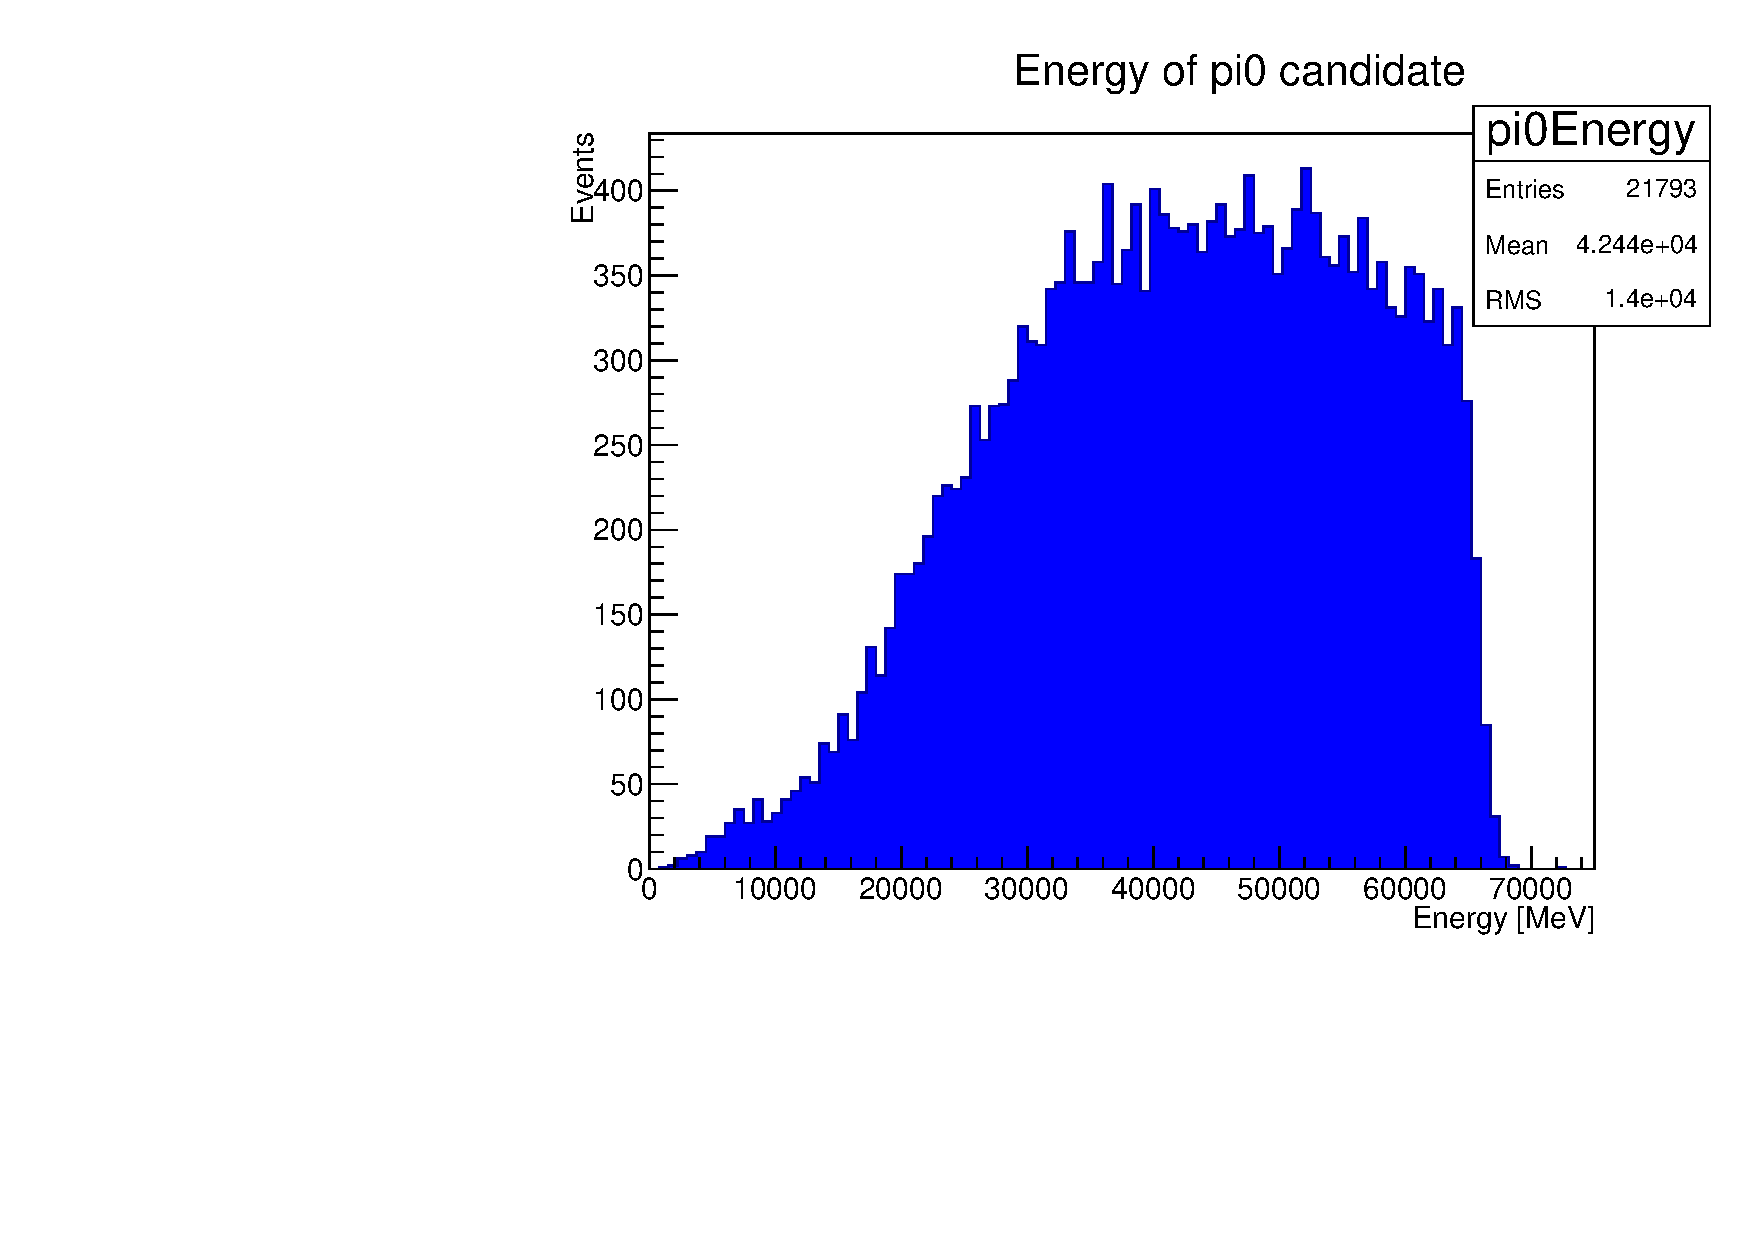
\includegraphics[width=\textwidth]{energypi0}
\end{subfigure}
\begin{subfigure}{0.5\textwidth}
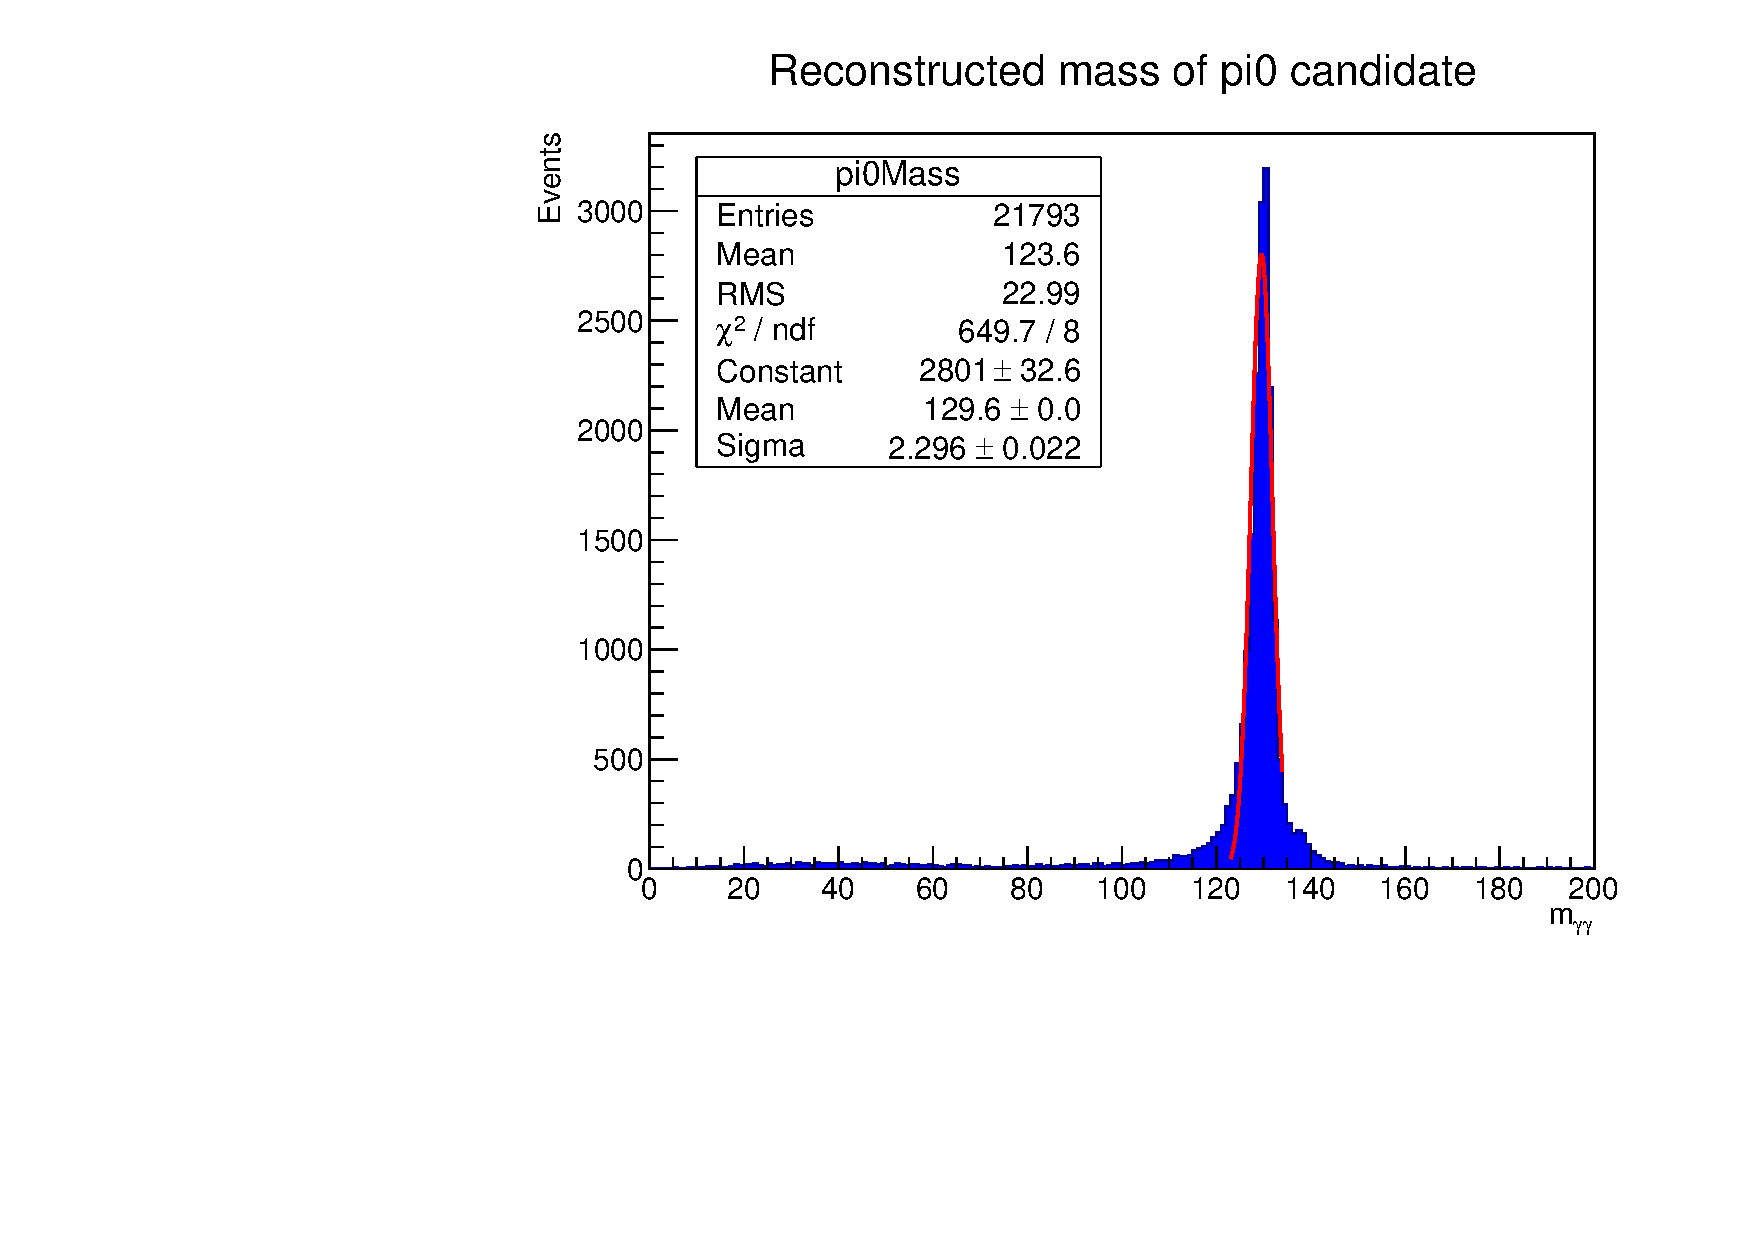
\includegraphics[width=\textwidth]{masspi0}
\end{subfigure}\\
\begin{subfigure}{\textwidth}
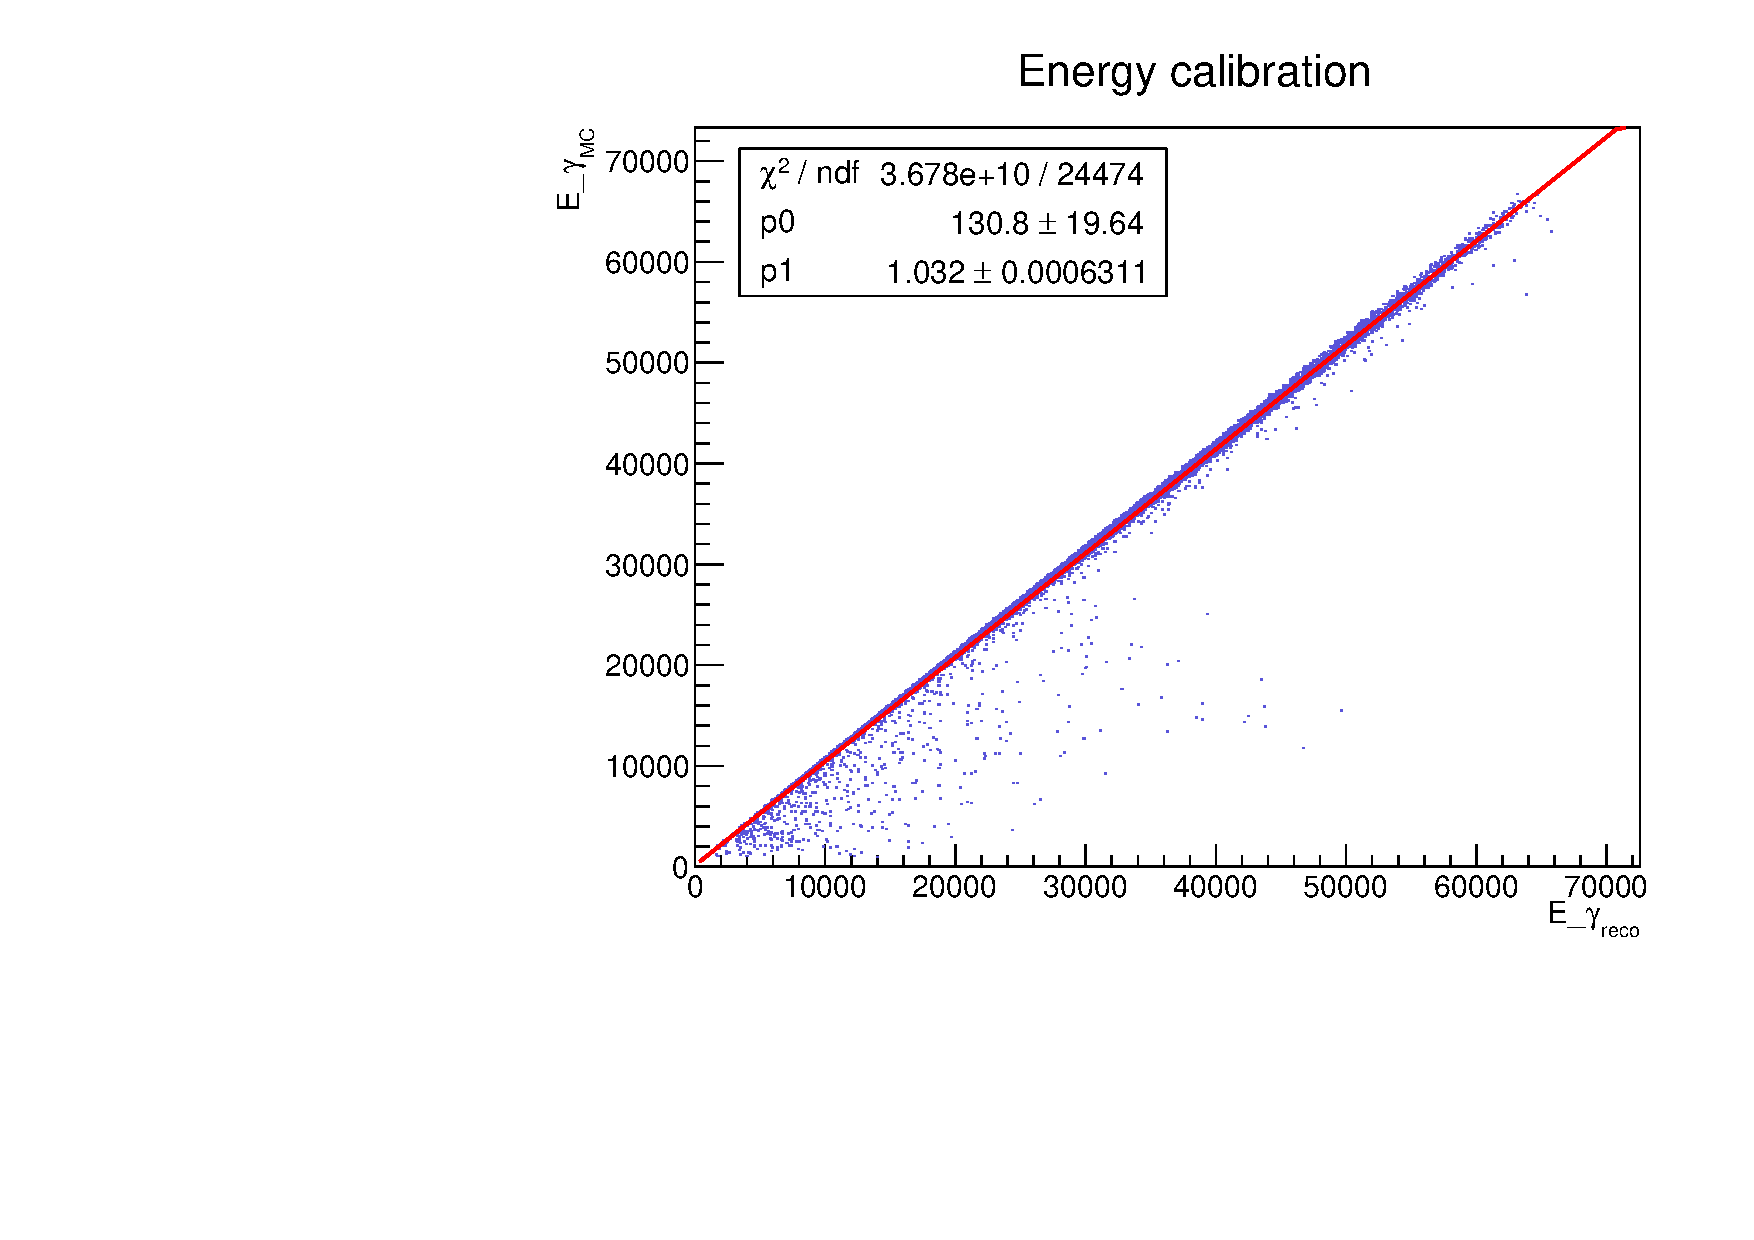
\includegraphics[width=\textwidth,height=150pt]{calibpi0}
\end{subfigure}
\caption{Top: histograms of the reconstructed $\pi^0$ candidate mass and energy. Bottom:
Fit of the $E_{reco}$ vs. $E_{MC}$ slope for the verification of the
calibration constants.}\label{pi0validation}
\end{figure}


